\begin{frame}
\frametitle{Task 4: Theory}
The excitation current 
\begin{equation}
\mathbf{I} =[A_1e^{j\Phi_1} A_2e^{j\Phi_2} \dots A_{N-1}e^{j\Phi_{N-1}}],
\end{equation}
 element positions $\{\mathbf{r}_i\}_{i=1}^N$

Far field function of the array (assuming identical elements)


\begin{equation}
\mathbf{G}_A(\theta, \phi) = \sum_{n=1}^N A_ne^{j\phi_n}(G_{\theta}\hat{\theta} + G_{\phi}\hat{\phi}) e^{jk\mathbf{r}_n\dot{\hat{r}}}.
\end{equation}
Which can be written as 
\begin{equation}
\mathbf{G}_A(\theta, \phi) = \mathbf{G}(\theta, \phi) \cdot AF
\end{equation}


\end{frame}



\begin{frame}
\frametitle{Task 4: Results}
\begin{figure}[h]
\centering
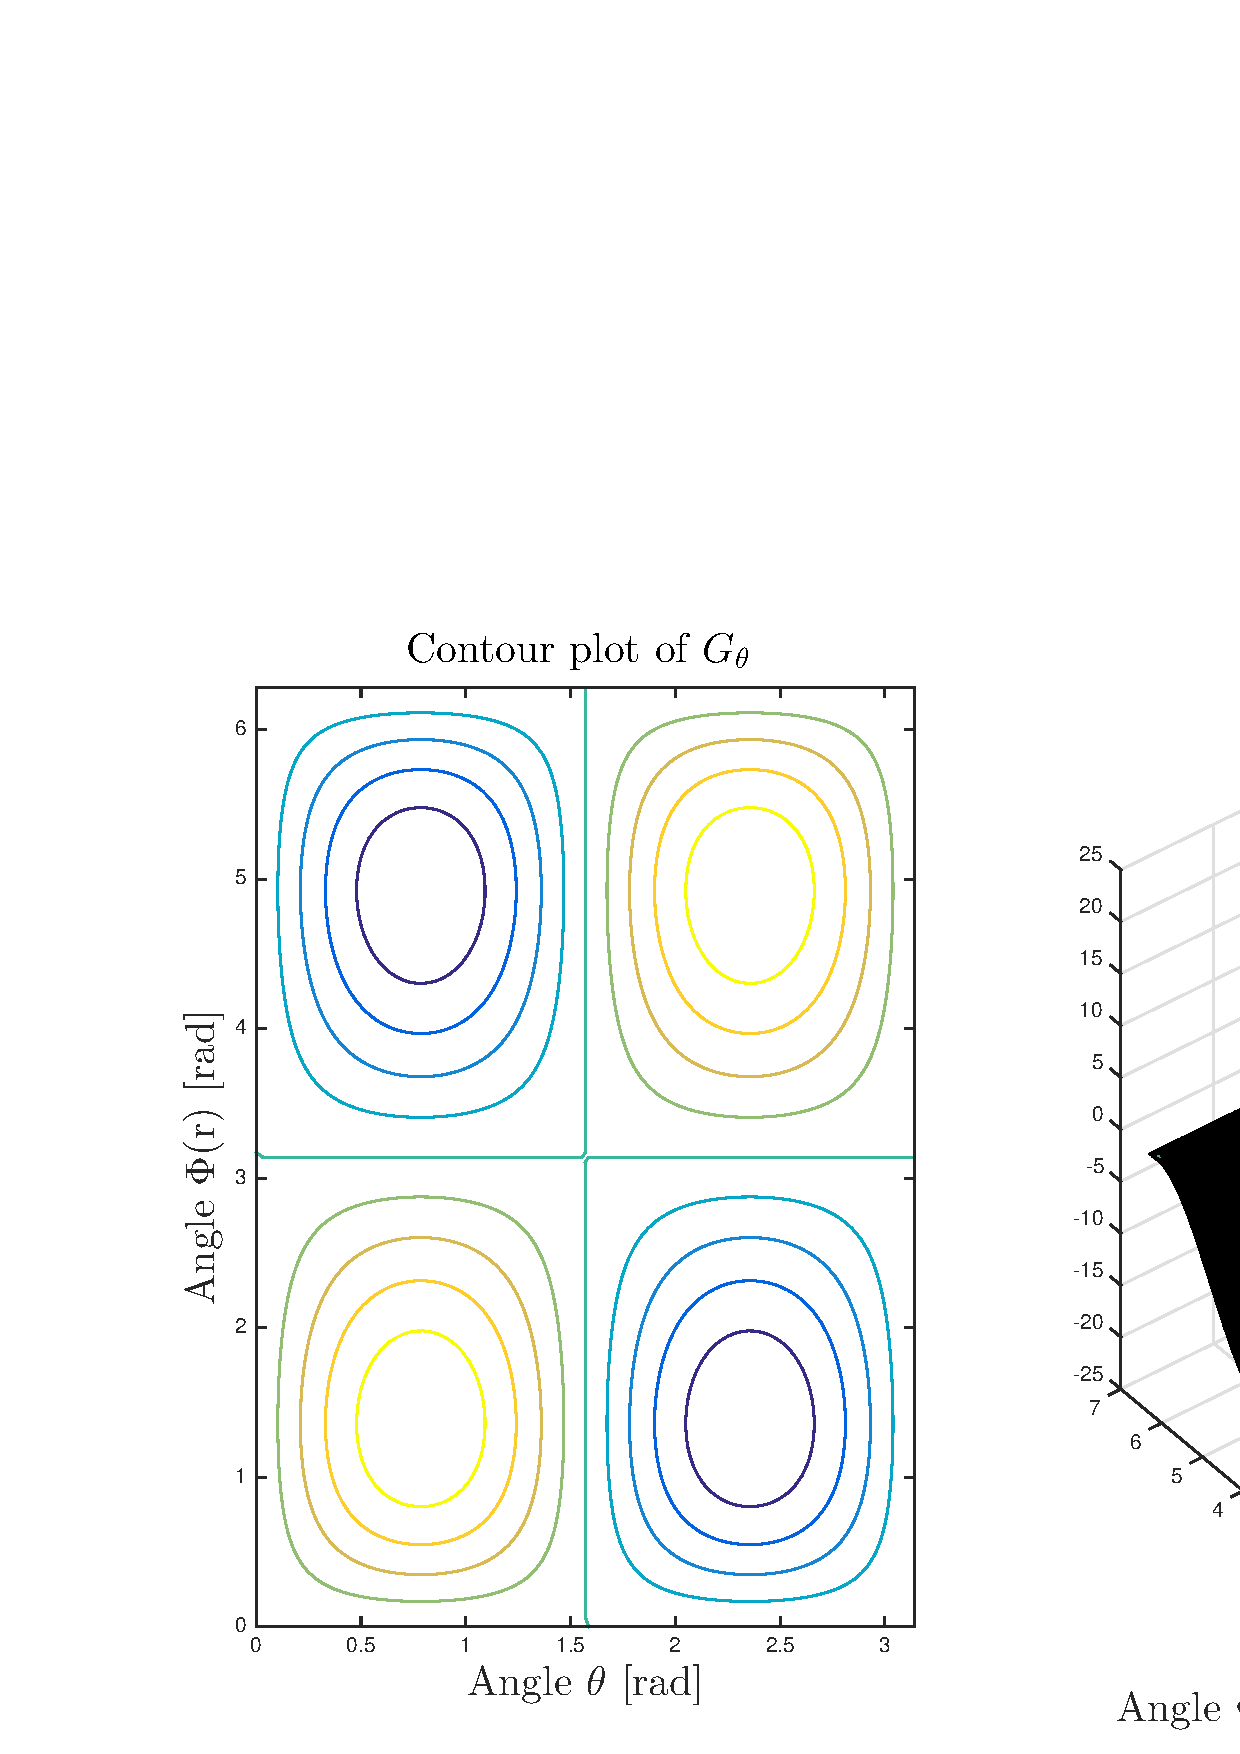
\includegraphics[scale=0.3]{/Users/marikasvensson/Documents/MATLAB/MicroProject/finished/task4/Gth.png}
\caption{This figure shows $G_\theta$ as a function of $\theta$ and $\phi$}
\label{task4:Gth}
\end{figure}




\end{frame}


\begin{frame}
\frametitle{Task 4: Results}
\begin{figure}[h]
\centering
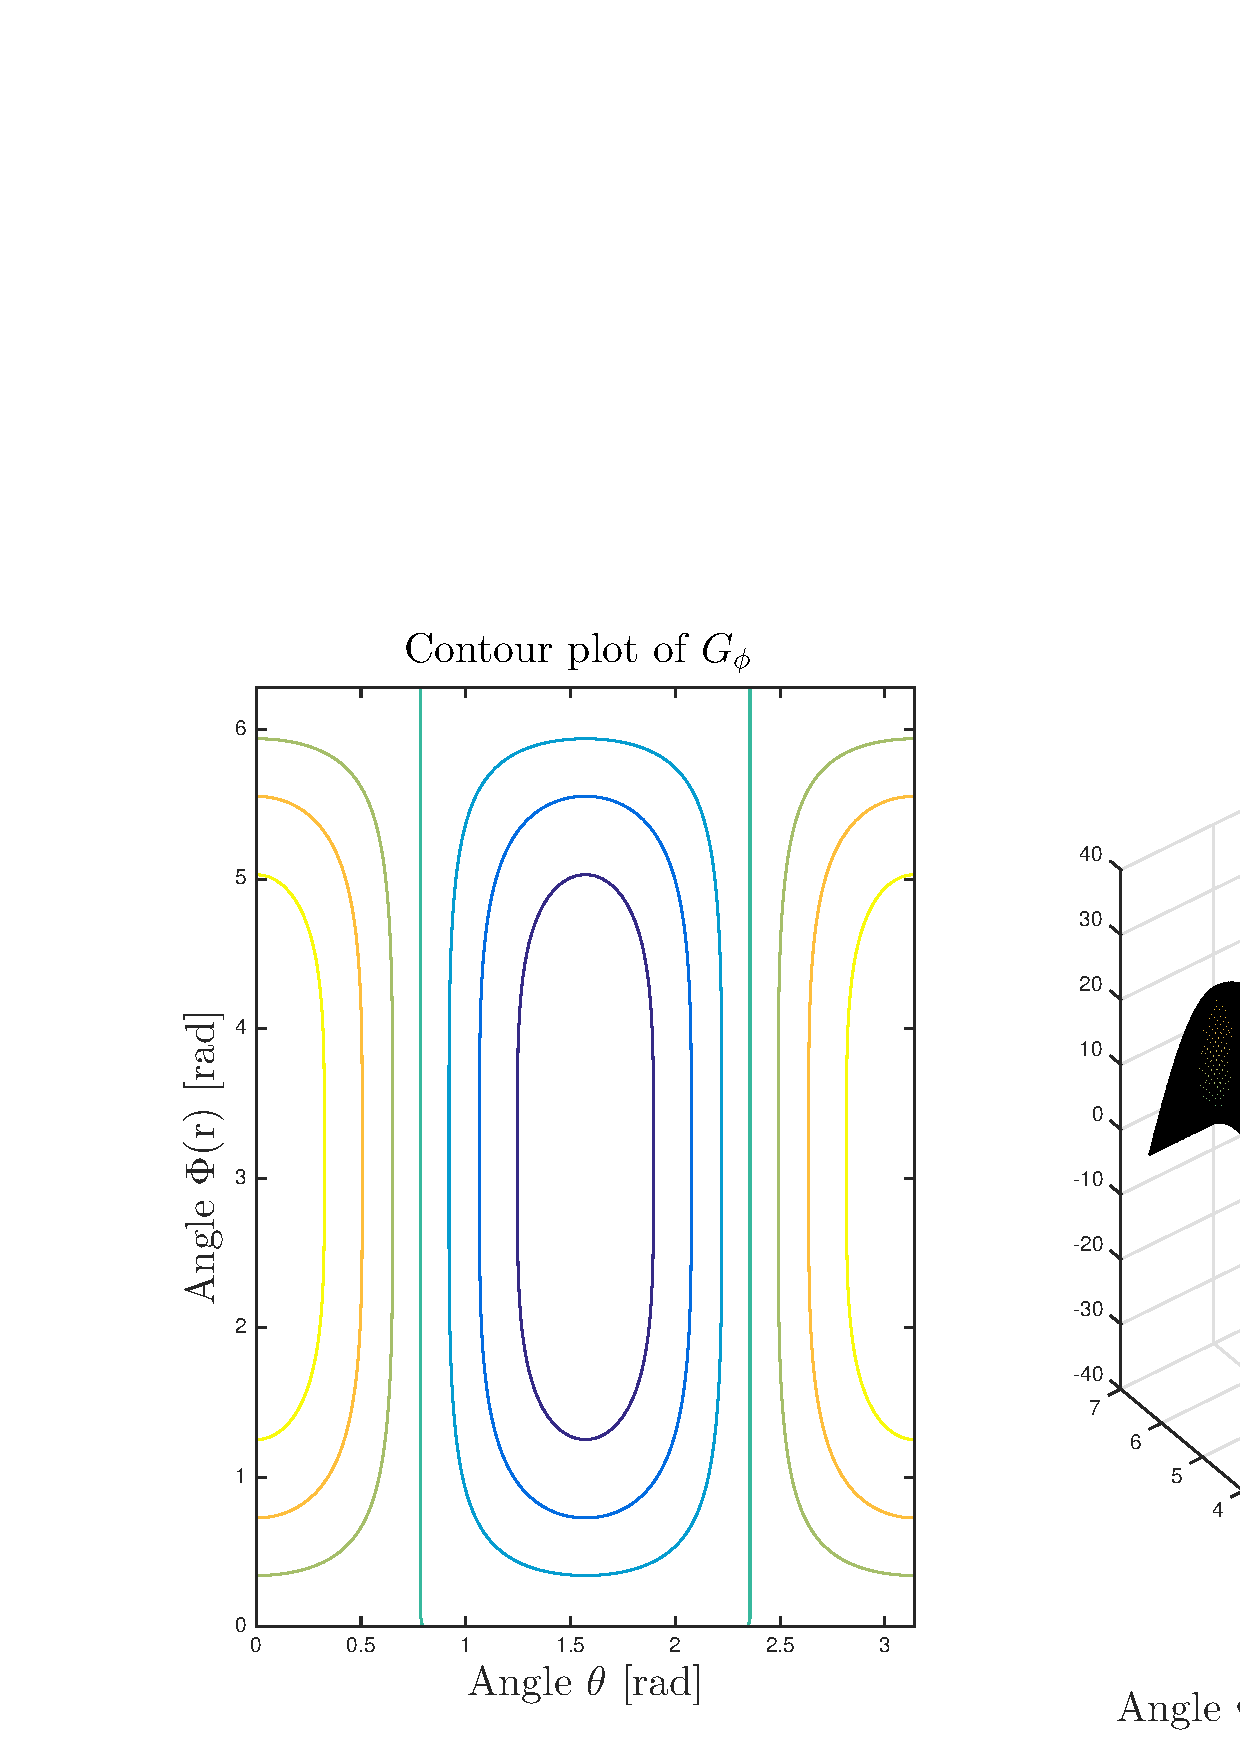
\includegraphics[scale=0.3]{/Users/marikasvensson/Documents/MATLAB/MicroProject/finished/task4/Gphi.png}
\caption{This figure shows $G_\phi$ as a function of $\theta$ and $\phi$}
\label{task4:Gphi}
\end{figure}


\end{frame}